\chapter{Conception}

\section{Interface graphique}

Comme précisé précédemment, notre programme se présente sous la forme d'un plugin \imj. Il a été réalisé grâce à la bibliothèque Swing de \java ~pour l'interface graphique. Celle-ci offre la possibilité de créer des interfaces graphiques identiques quelque soit le système d'exploitation sous-jacent.\\
Nous avons donc créé une série d'outils graphiques (boutons, listes, labels) pour l'interaction avec l'utilisateur. Dans une fenêtre, ces outils sont disposés en lignes ou en colonnes dans des boîtes (panels). Les boîtes peuvent s'imbriquer les unes dans les autres afin d'obtenir des structures plus complexes et un meilleur rendu visuel. \\
L'interface du plugin est simple, elle prend la forme d'une fenêtre composée d'un menu déroulant, dans lequel se trouvent les différents algorithmes, et de quatre boutons. \\

\subsection{Les panels}

Notre interface est composée de quatre panels différents (voir Figure \ref{panels}) :
\begin{itemize}

\item Le panel en haut de la fenêtre (\textbf{panel1}) contient la combobox pour le choix de l'algorithme. 
\item Le panel du milieu (\textbf{panel2}) est vide au lancement du plugin et son contenu s'affiche en fonction de l'algorithme de piquage choisi. Il contient 4 sous-panels :
\begin{itemize}
\item Le premier sous-panel (\textbf{infoPanel}) contient une zone de texte visant à guider l'utilisateur sur la manière de lancer la procédure de piquage choisie. 
\item Le deuxième sous-panel se situe au milieu de panel2 et porte un nom différent suivant l'algorithme choisi : il va se nommer \textbf{iterationPanel} pour Dilate Difference, \textbf{sigmaPanel} pour Difference of Gaussian et \textbf{radiusPanel} pour Image Correlation. Ces sous-panels contiennent deux ou trois TextFields (zones de texte à une seule ligne) pour que l'utilisateur puisse entrer les valeurs des paramètres nécessaires au bon fonctionnement des algorithmes. 
\item Le troisième sous-panel (\textbf{widthNoisePanel}) quand à lui contient deux TextFields pour les paramètres \textbf{Square width} et \textbf{Noise Tolerance} sur lesquels nous reviendrons par la suite. 
\item Le dernier sous-panel (\textbf{debugCropPanel}) contient deux checkboxs pour les modes de debug et crop (voir plus loin dans le rapport). 
\end{itemize}
\item Le panel en bas de la fenêtre (\textbf{panel3}) contient quatre boutons qui permettent à l'utilisateur de faire fonctionner le plugin. 
\item Le panel principal (\textbf{mainPanel}) contient tous les panels cités précédemment. Sa taille détermine celle de la fenêtre du plugin. 
\end{itemize}

\begin{figure}[!h] 
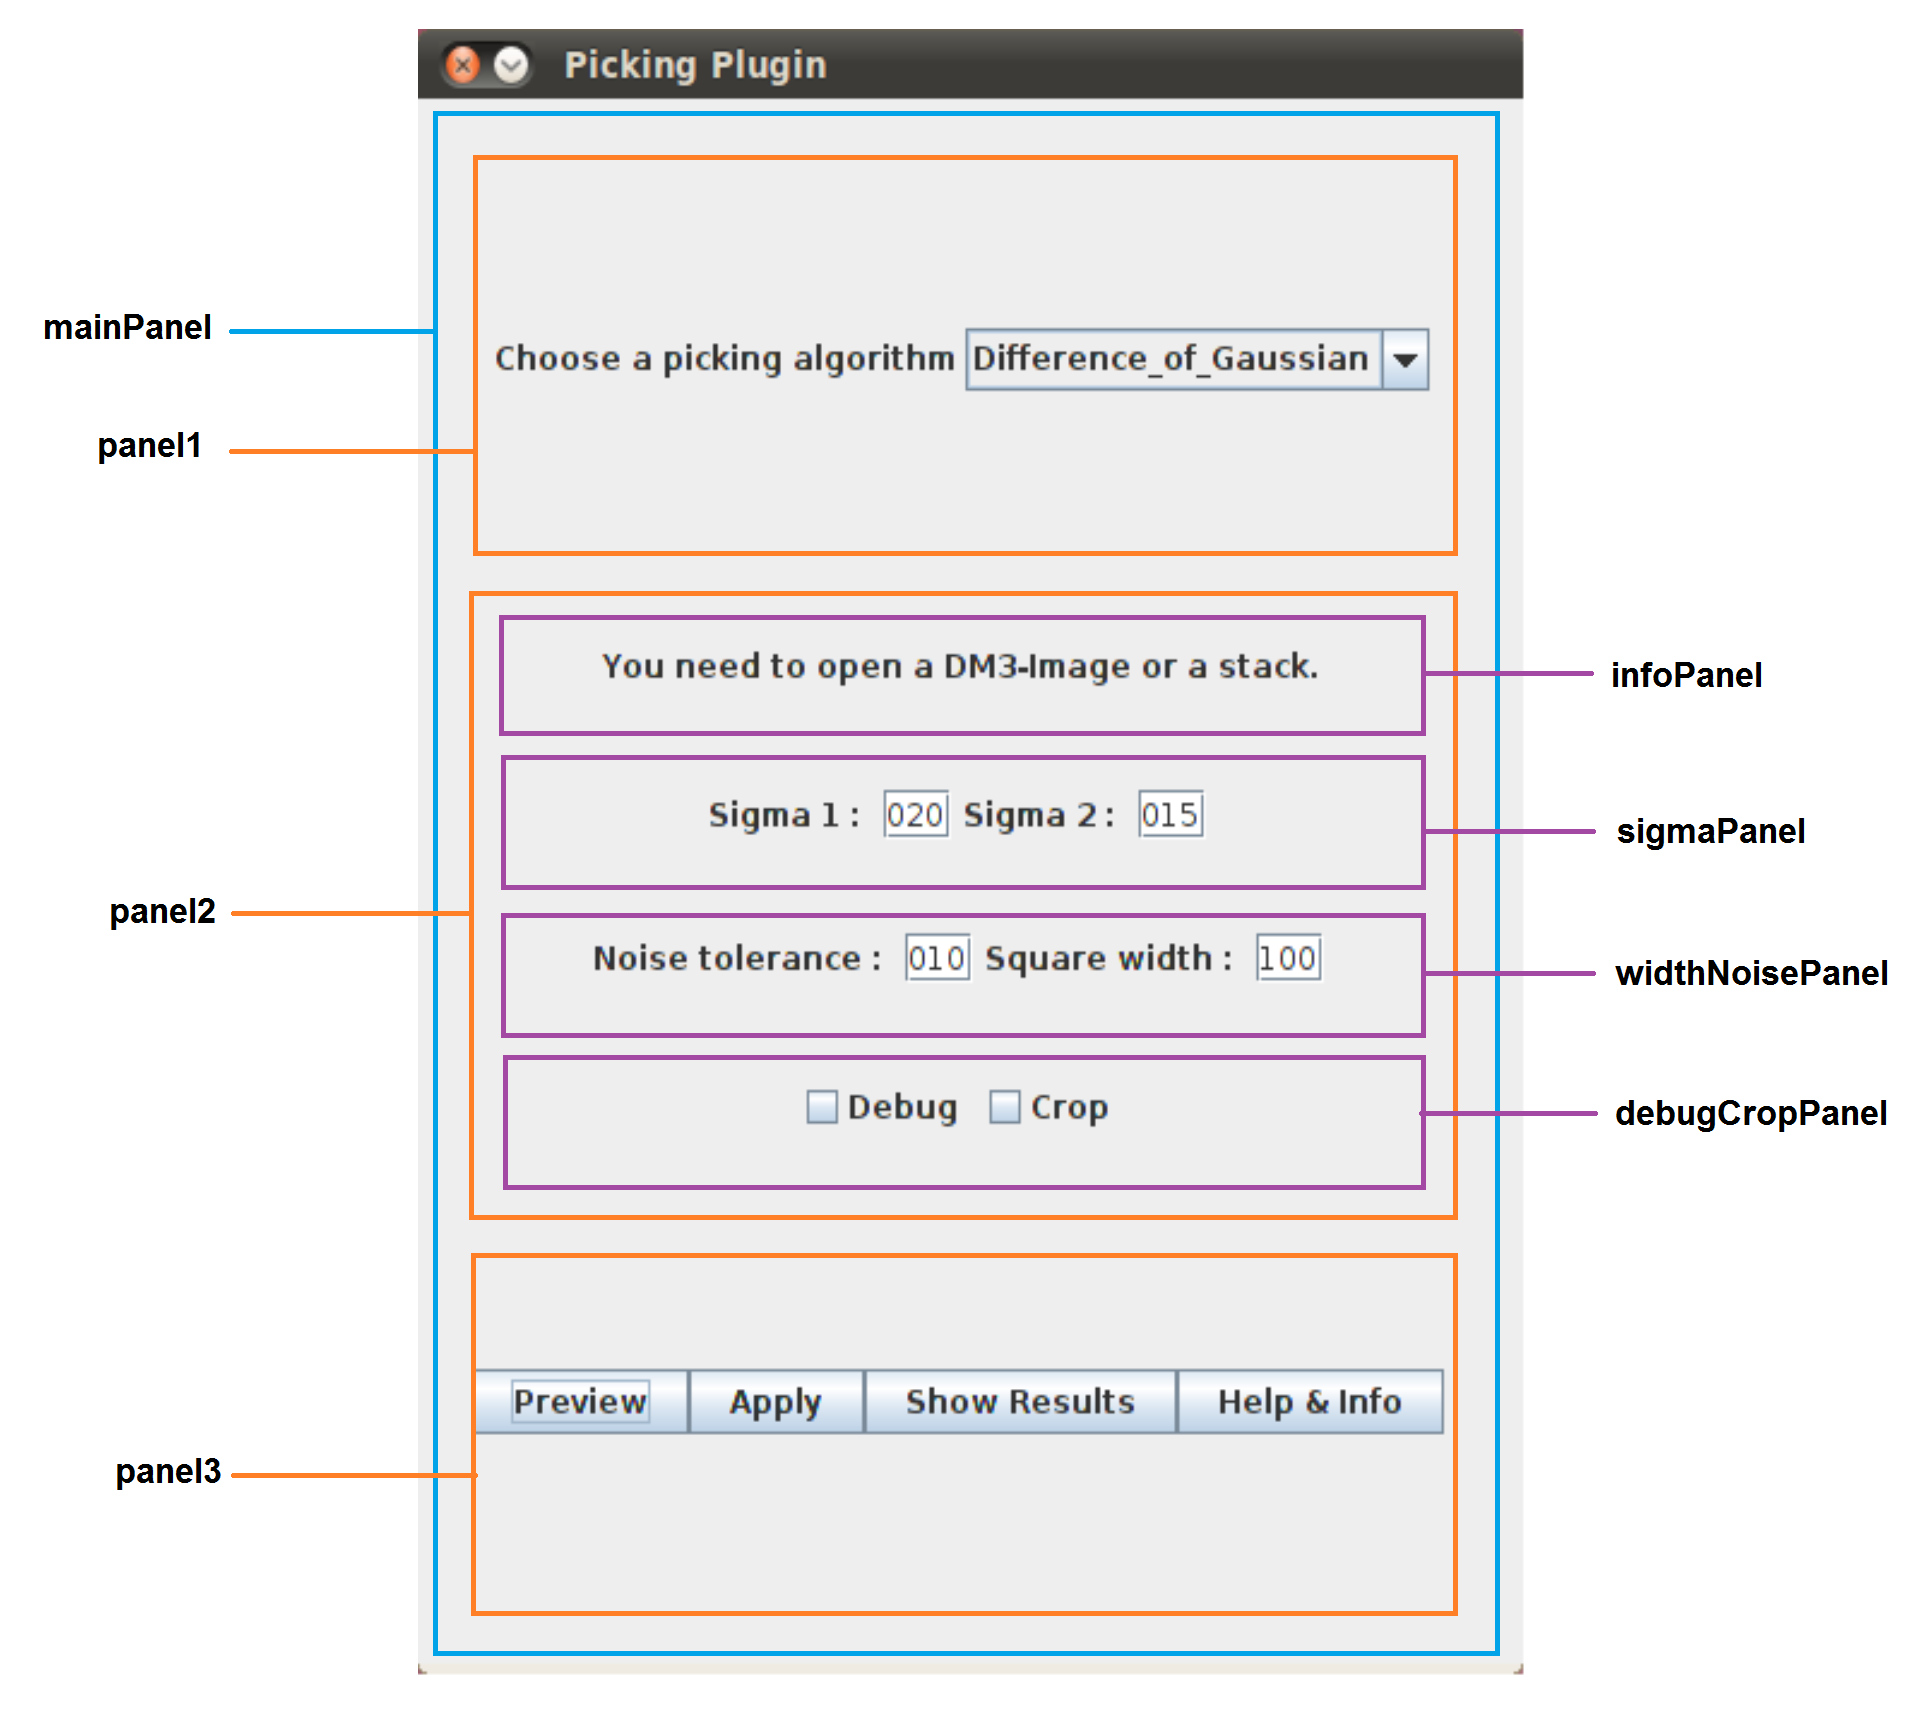
\includegraphics[width=1\textwidth]{plugin3-1.png}
\caption{Organisation des panels pour l'algorithme Difference of Gaussian}
\label{panels}
\end{figure}

\subsection{Les boutons}

Les boutons doivent répondre aux clics de la souris et lancer une série d'actions correspondantes en fonction de l'algorithme de piquage choisi par l'utilisateur :

\begin{itemize}
\item Le bouton \textbf{Preview} permet de tester l'algorithme sélectionné sur une seule image du stack.
\item Le bouton \textbf{Apply} permet d'appliquer l'algorithme sur l'ensemble du stack, lorsque l'utilisateur a défini les paramètres qu'il souhaite appliquer.
\item Le bouton \textbf{Help \& Info} est une aide d'utilisation du plugin.
\item Le bouton \textbf{Save Results} permet de sauvegarder le tableau de coordonnées des particules sélectionnées.% avec l'aide d'\imj.  
\end{itemize}
Pour que le plugin puisse fonctionner, l'utilisateur devra au préalable avoir ouvert un stack d'image à l'aide d'\imj.

\subsection{Algorithmes et paramètres d'entrée}

Lorsque l'utilisateur sélectionne un algorithme dans le menu déroulant, il doit ensuite choisir plusieurs paramètres.
Certains sont communs à tous. Il s'agit de la \textbf{Noise Tolerance} et de la largeur du carré que l'utilisateur souhaite utiliser pour faire le stack des particules sélectionnées (\textbf{Square width}) s'il décide de se servir de la fonction \texttt{crop} du plugin.

\subsubsection{Image Correlation}

Le principe de cette méthode est de comparer une image contenant un cercle avec l'image sur laquelle on veut sélectionner les particules. On obtient alors une nouvelle image sur laquelle on peut voir des cercles correspondant aux particules de l'image de base qui ont à peu près le même diamètre que le cercle dessiné précédemment. Ici, on fait varier la taille du cercle afin de sélectionner des particules de différentes tailles.\\
\noindent
Pour cet algorithme de piquage, l'utilisateur doit entrer le rayon minimal/maximal (\textbf{radius min, radius max}) des particules à sélectionner, ainsi que la valeur de l'incrémentation (\textbf{radius inc}). Pour un résultat optimal, avant de lancer la sélection des particules avec cet algorithme, l'utilisateur devra traiter l'image pour éliminer un maximum de bruit de fond (utilisation de filtres, modification du contraste/luminosité, sélection des contours, application d'un threshold).

\subsubsection{Difference of Gaussian}

La différence de Gauss est une technique qui consiste en la soustraction d'une version floutée de l'image d'origine à une autre version moins floutée de cette même image.\\
Ici, l'utilisateur doit entrer les valeurs de \textbf{sigma1} et \textbf{sigma2} qui vont être utilisées pour appliquer les filtres gaussiens.

\subsubsection{Dilate Difference}

Cette méthode repose sur le même principe que la différence de Gauss à ceci près que l'image d'origine n'est pas floutée mais on lui applique un certain nombre de cycles de dilatation, on obtient alors des particules grossies.\\
Dans le cas de la sélection de cet algorithme, l'utilisateur devra entrer les nombres de cycles de dilatation qu'il souhaite appliquer(\textbf{iteration1, iteration2}).

\section{Paramètres de sortie}

Lorsque l'utilisateur a choisi un algorithme et l'a appliqué au stack, le plugin renvoie (si l'utilisateur le demande) un tableau contenant les coordonnées (\emph{x} et \emph{y}) des particules sélectionnées, ainsi que leur position dans le stack (\emph{slice}). Il pourra par la suite le sauvegarder gr\^ace au menu d'\imj. \\
De plus, si l'utilisateur en fait la demande, un stack contenant autant d'images que de particules sélectionnées est créé.

\section{Les classes}

Le programme est divisé en seize classes distinctes:
\begin{list}{•}
\item Une première partie regroupe six classes qui permettent de gérer l'interface graphique.
\item
\item Une seconde partie regroupe les algorithmes de piquage, elle est composée de quatre classes.
\item La classe \texttt{AlgoFactory} sert de pivot au programme en fonction du choix d'algorithme de l'utilisateur (adaptation de l'interface et algorithme de piquage).
\item La classe \texttt{Attributes} est un singleton (instanciable qu'une seule et unique fois) et contient tous les paramètres à entrer par l'utilisateur pour faire fonctionner les algorithmes.
\item La classe \texttt{Cropper} est une fonction subsidiaire du piquage permettant de créer un stack dans lequel chaque image contient une particule piquée (si l'utilisateur le demande).
\item La classe \texttt{FFTMath} contient la méthode permettant de faire la Corrélation d'images.
\item Les classes \texttt{About} et \texttt{InfoHelp} contiennent des informations et une aide sur l'utilisation du plugin.
\end{list}

\subsection{Les classes de l'interfaces}

La classe \texttt{Pick\_EM} fait le lien entre \imj ~et la classe \texttt{PickFrame} qui est une JFrame, elle permet de créer l'interface graphique.\\
Vient ensuite la classe \texttt{PickPanel} qui permet d'adapter l'interface en fonction de l'algorithme. En découlent \texttt{PanelDilateDiff}, \texttt{PanelDoG} et \texttt{PanelImCorr} pour leurs algorithmes respectifs (Dilate Difference, Difference Of Gaussian et Image Correlation).

\subsection{Les classes des algorithmes}

La classe \texttt{Picker} est utilisée pour appeler les algorithmes. Les algorithmes étant \texttt{DialteDiff}, \texttt{DoG} et \texttt{ImCorr}.
Pour faire fonctionner ces algorithmes, la classe \texttt{Attributes} renvoie les valeurs des paramètres entrés par l'utilisateur.
